\section{\method{} 方法}
\label{sec:ink-functional-geometry}

\begin{figure}[!htbp]
  \centering
  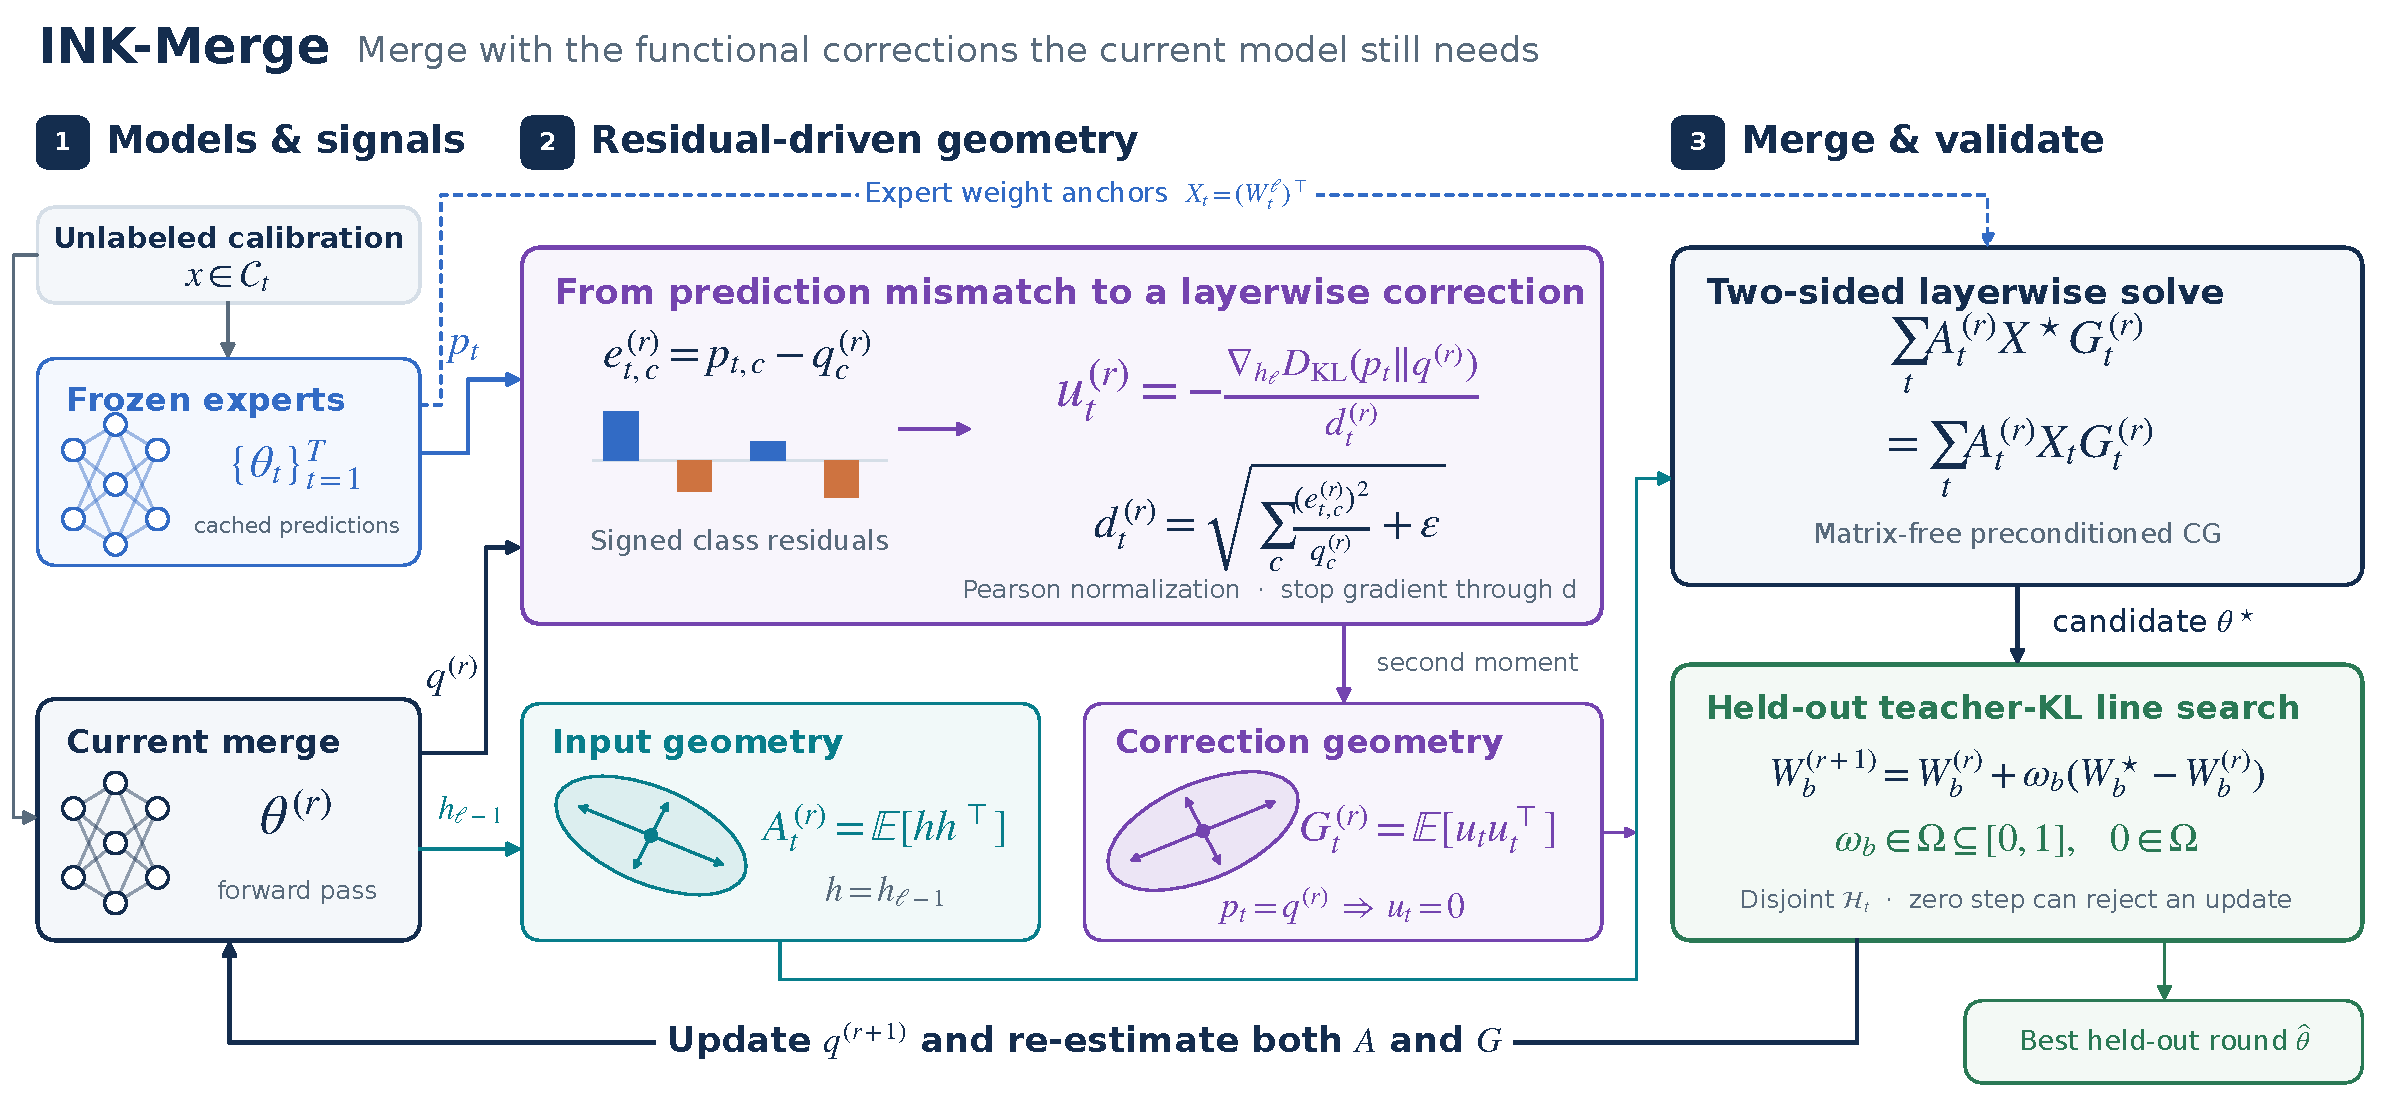
\includegraphics[width=\linewidth]{figures/ink_method_overview.pdf}
  \caption{\method{} 方法总览，对应式~(\ref{eq:ink-dynamic-geometry})。\textbf{1}~冻结专家提供软预测 $p_t$ 与权重锚点 $X_t$，当前模型 $\theta^{(r)}$ 给出 $q^{(r)}$ 与激活 $h_{\ell-1}$。\textbf{2}~类别残差经教师--学生 KL 负梯度与 Pearson 归一化得到层级修正 $u_t^{(r)}$；其二阶矩 $G_t^{(r)}$ 与输入二阶矩 $A_t^{(r)}$ 构成随 $\theta^{(r)}$ 变化的双侧几何。\textbf{3}~矩阵自由预条件共轭梯度求解候选权重，留出教师 KL 选择块级步长（含零步长拒绝），随后重估 $A$ 与 $G$ 并迭代，最终取留出 KL 最小的轮次。图中省略层下标 $\ell$，$G_t^{(r)}$ 简记 $G_{t,\mathrm{ink}}^{\ell,(r)}$，椭圆仅示意几何方向。}
  \label{fig:ink-overview}
\end{figure}


现有几何感知合并方法通常为每个专家估计固定的重要性几何 $C_t(\theta_t,\mathcal D_t)$。然而，模型更新后，它与不同专家之间尚未消除的功能差异也会改变，因此固定几何不能准确描述当前仍需保留或恢复的功能方向。\method{} 将几何写成式~(\ref{eq:ink-dynamic-geometry})，根据专家模型与当前合并模型之间的预测残差，在每一轮重新估计任务特定的功能修正几何。具体而言，我们将教师--学生 KL 关于层表示的归一化负梯度定义为局部功能修正向量，并以其二阶矩刻画输出侧几何。该几何与输入激活二阶矩共同构成 Kronecker 因子化度量，用于求解逐层参数合并。

\subsection{从预测残差到功能修正方向}

固定任务 $t$、输入 $x$ 和当前轮次 $r$，简写 $p_{t,c}=p_t(c\mid x)$、$q_c^{(r)}=q^{(r)}(c\mid x)$。首先定义专家与当前模型在类别 $c$ 上的预测残差
\begin{equation}
  e_{t,c}^{(r)}(x)
  =
  p_{t,c}-q_c^{(r)}.
  \label{eq:ink-prediction-residual}
\end{equation}
对第 $\ell$ 层表示 $h_\ell$，定义当前模型的类别得分
\begin{equation}
  s_c^{\ell,(r)}(x)
  =
  \nabla_{h_\ell}\log q^{(r)}(c\mid x).
\end{equation}
由于得分恒等式
\begin{equation}
  \sum_c q_c^{(r)}s_c^{\ell,(r)}(x)=0,
\end{equation}
教师--学生 KL 关于层表示的负梯度可以直接写为
\begin{align}
  -\nabla_{h_\ell}D_{\mathrm{KL}}(p_t\|q^{(r)})
  &= \sum_c p_{t,c}s_c^{\ell,(r)}(x) \\
  &= \sum_c \left(p_{t,c}-q_c^{(r)}\right)
     s_c^{\ell,(r)}(x).
  \label{eq:ink-kl-score-identity}
\end{align}
式~(\ref{eq:ink-kl-score-identity}) 将每个类别上的预测残差映射为层表示空间中的功能修正方向：$p_{t,c}>q_c^{(r)}$ 的类别沿其得分方向增强，$p_{t,c}<q_c^{(r)}$ 的类别则沿相反方向抵消。

\subsection{Pearson 归一化与局部修正}

为避免当前模型在某些类别上给出很小概率时产生过大的样本尺度，定义 Pearson 归一化项
\begin{equation}
  d_t^{(r)}(x)
  =
  \sqrt{
    \sum_c
    \frac{\left(p_{t,c}-q_c^{(r)}\right)^2}{q_c^{(r)}}
    +\varepsilon
  }.
  \label{eq:ink-pearson-normalizer}
\end{equation}
根号内除 $\varepsilon$ 外即为 $p_t$ 相对于 $q^{(r)}$ 的 Pearson-$\chi^2$ 散度。归一化的样本级修正向量为
\begin{align}
  u_t^{\ell,(r)}(x)
  &=
  \frac{
    \sum_c\left(p_{t,c}-q_c^{(r)}\right)
    s_c^{\ell,(r)}(x)
  }{d_t^{(r)}(x)} \\
  &=
  -\frac{
    \nabla_{h_\ell}D_{\mathrm{KL}}(p_t\|q^{(r)})
  }{d_t^{(r)}(x)}.
  \label{eq:ink-layer-correction}
\end{align}
该归一化保留各类别残差的相对符号与方向，同时使不同置信度尺度下的样本更可比较。实现时，我们对归一化教师 KL 做一次反向传播，并对分母停止梯度；反向钩子若收集到 $-u$，不会改变后续的 $uu^\top$。

\subsection{动态输出修正几何}

为了识别任务 $t$ 在不同样本上持续要求修正的功能子空间，定义输出侧二阶矩
\begin{equation}
  \boxed{
  G_{t,\mathrm{ink}}^{\ell,(r)}
  =
  \mathbb E_{x\sim\mathcal D_t}
  \left[
    u_t^{\ell,(r)}(x)u_t^{\ell,(r)}(x)^\top
  \right]
  }.
  \label{eq:ink-output-geometry}
\end{equation}
$G_{t,\mathrm{ink}}^{\ell,(r)}$ 为半正定矩阵，刻画任务 $t$ 在该层尚待修正方向的强度与相关结构。它同时依赖专家分布 $p_t$ 和当前分布 $q^{(r)}$：当两者匹配时，修正信号消失；当当前模型更新时，几何也随之改变。这与只描述专家附近局部敏感度的固定 Fisher 因子不同。

\subsection{Kronecker 因子化逐层合并}
\label{sec:ink-kronecker-merging}

考虑第 $\ell$ 个线性层。记专家 $t$ 的权重为 $W_t^\ell\in\mathbb R^{d_{\mathrm{out}}\times d_{\mathrm{in}}}$，并令 $X_t^\ell=(W_t^\ell)^\top$。输入侧几何由当前合并模型在任务数据上的激活二阶矩给出：
\begin{equation}
  A_t^{\ell,(r)}
  =
  \mathbb E_{x\sim\mathcal D_t}
  \left[h_{\ell-1}h_{\ell-1}^\top\right].
  \label{eq:ink-input-geometry}
\end{equation}
$A_t^{\ell,(r)}$ 描述该任务实际访问的输入方向，$G_{t,\mathrm{ink}}^{\ell,(r)}$ 描述尚未消除的输出功能分歧。二者定义双侧目标
\begin{equation}
  \mathcal J_\ell(X)
  =
  \frac12\sum_{t=1}^T
  \operatorname{tr}
  \left[
    (X-X_t^\ell)^\top
    A_t^{\ell,(r)}
    (X-X_t^\ell)
    G_{t,\mathrm{ink}}^{\ell,(r)}
  \right].
  \label{eq:ink-layer-objective}
\end{equation}
令梯度为零，得到正规方程
\begin{equation}
  \boxed{
  \sum_{t=1}^T
  A_t^{\ell,(r)}X^{\ell,\star}G_{t,\mathrm{ink}}^{\ell,(r)}
  =
  \sum_{t=1}^T
  A_t^{\ell,(r)}X_t^\ell G_{t,\mathrm{ink}}^{\ell,(r)}
  }.
  \label{eq:ink-normal-equation}
\end{equation}
我们把左侧实现为矩阵--矩阵线性算子，以对角预条件共轭梯度求解，不显式构造完整 Kronecker 矩阵。专家锚点 $X_t^\ell$ 保留参数目标位置；输出二阶矩虽把单个修正表示为功能轴，各类别预测残差的正负号已经在形成 $u$ 时决定不同得分方向如何增强或抵消。

\subsection{迭代重估与保守更新}
\label{sec:ink-iterative-update}

预测残差导出的功能修正、输入激活与输出修正几何都依赖当前模型。逐层求解式~(\ref{eq:ink-normal-equation}) 得到候选权重 $W^\star$ 后，对每个 Transformer 块采用保守插值
\begin{equation}
  W_b^{(r+1)}
  =
  W_b^{(r)}
  +
  \omega_b^{(r)}
  \left(W_b^\star-W_b^{(r)}\right),
  \qquad
  \omega_b^{(r)}\in\Omega\subseteq[0,1].
  \label{eq:ink-conservative-step}
\end{equation}
步长由互不重叠的无标签留出样本上的平均教师 KL 选择。候选集合始终包含 $0$，因此不能改善行为目标的块更新可以被完全拒绝。每轮接受后，算法围绕新的 $q^{(r+1)}$ 重新估计 $A_t^{\ell,(r+1)}$ 与 $G_{t,\mathrm{ink}}^{\ell,(r+1)}$；最终从初始化和所有轮次中选择留出教师 KL 最小者。

\begin{algorithm}[t]
  \DontPrintSemicolon
  \SetKwInput{KwIn}{输入}
  \SetKwInput{KwOut}{输出}
  \SetKw{KwTo}{至}
  \SetKwFor{For}{对于}{执行}{结束}
  \SetKwIF{If}{ElseIf}{Else}{如果}{则}{否则如果}{否则}{结束}
  \KwIn{专家 $\{\theta_t\}_{t=1}^T$；各任务无标签集合 $\{\mathcal C_t,\mathcal H_t\}$；轮数 $R$；步长 $\Omega$}
  \KwOut{合并模型 $\widehat\theta$}
  缓存每个专家在 $\mathcal C_t\cup\mathcal H_t$ 上的软预测 $p_t$\;
  以公共子空间合并初始化 $\theta^{(0)}$，并将其加入候选集 $\mathcal Q$\;
  \For{$r\leftarrow0$ \KwTo $R-1$}{
    在 $\theta^{(r)}$ 上计算 $q^{(r)}$、$A_t^{\ell,(r)}$ 和 $G_{t,\mathrm{ink}}^{\ell,(r)}$\;
    对每个线性层，以预条件共轭梯度求解式~(\ref{eq:ink-normal-equation})，得到 $W^{\ell,\star}$\;
    在 $\mathcal H_t$ 上以平均教师 KL 选择全局步长，并逐块细化 $\omega_b^{(r)}\in\Omega$\;
    按式~(\ref{eq:ink-conservative-step}) 得到 $\theta^{(r+1)}$，并加入 $\mathcal Q$\;
    \If{所有块的步长均为 $0$ 或相对更新量低于阈值}{停止}
  }
  $\widehat\theta\leftarrow\arg\min_{\theta\in\mathcal Q}\sum_t D_{\mathrm{KL}}(p_t\|q_\theta)$，其中 KL 在 $\mathcal H_t$ 上计算\;
  \caption{\method{} 的动态修正几何合并流程。}
  \label{alg:ink-merge}
\end{algorithm}


\subsection{与 MaTS 的关系}
\label{sec:ink-mats-comparison}

MaTS 用半正定矩阵 $C_t$ 表示专家 $t$ 的任务参数子空间，将合并写成
\begin{equation}
  \mathcal J_C(\theta)
  =
  \frac12\sum_{t=1}^T
  (\theta-\theta_t)^\top C_t(\theta-\theta_t),
  \qquad
  \left(\sum_tC_t\right)\theta^\star
  =
  \sum_tC_t\theta_t.
  \label{eq:ink-mats-subspace}
\end{equation}
对于线性层，K-FAC 近似令
\begin{equation}
  C_t^\ell\approx G_{t,F}^\ell\otimes A_t^\ell,
  \qquad
  G_{t,F}^\ell
  =
  \mathbb E\left[\delta_t^\ell(\delta_t^\ell)^\top\right],
\end{equation}
其中 $\delta_t^\ell$ 是任务损失对层输出的梯度。对应的双侧系统为
\begin{equation}
  \sum_tA_t^\ell X^\star G_{t,F}^\ell
  =
  \sum_tA_t^\ell X_t^\ell G_{t,F}^\ell.
  \label{eq:ink-mats-bilateral}
\end{equation}
Kronecker 乘积之和通常不能化为因子和的单个 Kronecker 乘积，因此 MaTS 将左侧视为线性算子，并用共轭梯度避免显式求逆。

\method{} 与 MaTS/K-FAC 在代数形式和求解器上最接近，但算子系数的语义与生命周期不同。MaTS 的 $G_{t,F}^\ell$ 是专家附近任务损失的输出梯度协方差，用固定任务子空间衡量哪些扰动敏感；\method{} 的 $G_{t,\mathrm{ink}}^{\ell,(r)}$ 则由专家--当前模型 KL 残差诱导，衡量当前模型尚需沿哪些功能方向修正，并在每次接受更新后改变。因此，我们复用的是双侧线性系统与共轭梯度这一计算骨架，而不是对同一个固定 Fisher 系统做更精确求解。
